\documentclass[tikz]{standalone}
\usepackage{tikz}
\usetikzlibrary{shapes,calc,arrows,through,intersections,angles}
\usepackage{xcolor}
\usepackage{pgfplots}
\pgfplotsset{compat=1.8}
\usepackage{nicefrac}

\begin{document}

%----Proper document------------------------------------------------------------

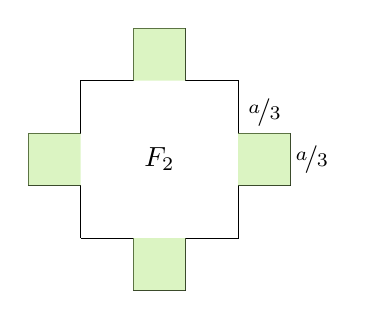
\begin{tikzpicture}[scale=2/3]
	\definecolor{limegreen}{RGB}{184,233,134}

	\draw (0,0) -- (1,0) -- (1,-1) -- (2,-1) -- (2,0) -- (3,0) -- (3,1) -- (4,1) -- (4,2) -- (3,2) -- (3,3) -- (2,3) -- (2,4) -- (1,4) -- (1,3) -- (0,3) -- (0,2) -- (-1,2) -- (-1,1) -- (0,1) -- (0,0);
	\fill [fill=limegreen, opacity=0.5] (1,0) -- (1,-1) -- (2,-1) -- (2,0) -- (1,0);
	\fill [fill=limegreen, opacity=0.5] (3,1) -- (4,1) -- (4,2) -- (3,2) -- (3,1);
	\fill [fill=limegreen, opacity=0.5] (1,3) -- (2,3) -- (2,4) -- (1,4) -- (1,3);
	\fill [fill=limegreen, opacity=0.5] (-1,1) -- (0,1) -- (0,2) -- (-1,2) -- (-1,1);
    
    \node at (3.5,2.4) {$\nicefrac{a}{3}$};
    \node at (4.4,1.5) {$\nicefrac{a}{3}$};
	\node at (1.5,1.5) {$F_2$};
\end{tikzpicture}

%-------------------------------------------------------------------------------

\end{document}
